\documentclass{standalone}
\usepackage{tikz}

\begin{document}

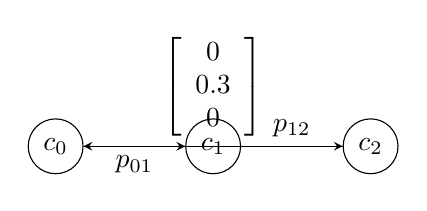
\begin{tikzpicture}[node distance=2cm, auto]

    % Define nodes
    \node (c0) [circle, draw] {\( c_0 \)};
    \node (c1) [circle, draw, right of=c0] {\( c_1 \)};
    \node (c2) [circle, draw, right of=c1] {\( c_2 \)};

    % Draw edges with labels
    \draw[-stealth] (c2) -- node[above] {$\left[\begin{array}{c} 0 \\ 0.3 \\ 0 \end{array}\right]$} (c0);
    \draw[-stealth] (c0) -- node[below] {$p_{01}$} (c1);
    \draw[-stealth] (c1) -- node[above] {$p_{12}$} (c2);

\end{tikzpicture}

\end{document}